\section{Introduction}
\label{sec:intro}

%%需要调研的部分:解答的问题,为什么我们关注多核的scalability问题。随着分布式系统的广泛普及,企业和用户的通用的做法是通过堆积更多的机器来获取更快的处理效率和速度。但是机器堆积的越多,网络带宽,耗电也越来越多,如何充分利用单台机器的多核资源成为很重要的课题。

%一方面,随着多核机器的广泛普及,如何充分利用多核资源成为非常重要的课题,另一方面,现有的很多我们希望充分利用单台机器上的资源,

%目前的现状,需求
As the prevalence of multicore chips,
it is foreseeable that tens to hundreds (even thousands) of cores on a single chip
will appear in the near future\cite{Borkar2007core}.
While utilizing multicore sources is still challenging
because of the difficulties of parallel programming.
Specifically, the thread-based model requires the programmer to manually
manage synchronization, load balancing, and locality, which is
often error-prone (e.g., races and deadlocks) or requires detailed
understanding of the underlying hardware.
An alternative approach is to rely on a runtime system for
concurrency management. 

MapReduce\cite{dean2004mapreduce}, 
for instance, is a promising programming model for clusters
to perform large-scale data processing
in a simple and efficient way.
In most cases, programmers only need to implement two functions:
map and reduce.
The runtime system spawns multiple threads that apply
these functions concurrently across the elements of the input
dataset. 
%The runtime spawns multiple threads to worker and 
%automatically manages synchronization, load balancing, 
%and locality in order to achieve efficient execution.
%which aggregates values in the key-value pairs according to the key.
And the programmer dose no need to control synchronization 
and schedule tasks manually.
%面向多核的MapReduce的相关工作
While initially MapReduce is implemented on clusters, Ranger
et al. have demonstrated the feasibility of running MapReduce
applications on shared memory multicore machines with 
Phoenix\cite{ranger2007phoenix}.
Other libraries such as Metis\cite{mao2010metis} 
, Tiled-mapreduce\cite{chen2010tiled} and MRPhi\cite{lu2013mrphi}, 
also show that MapReduce is a promising programming model 
for multicore platforms to take full advantage of  
processing resources.
Phoenix uses the pthread library to assign tasks 
among CPU cores and relies on
shared memory to handle inter-task communications.

%Phoenix存在的问题,scalability较差的原因
This work focuses on improving Phoenix\cite{ranger2007phoenix}'s scalability and performance.
On the one hand, 
While the original Phoenix performed well on small-scale systems,
we found that the runtime significantly underperformed on large-scale systems with multicores.
Specially, the performance will be better 
when the number of cores increases from 1 to 4, 
while the performance will be worse if using more than 4 cores. 
On the other hand,
there is a strict barrier between the Map and the
Reduce phase, which is bad for pipeline and hardware resource utilization.
To achieve scalable performance while retaining
the simplicity of the runtime-based approach, 
it becomes crucial to address these issues.

In contrast, Phoenix is a shared-memory version of
MapReduce targeted for multi-core and multiprocessor systems.
Phoenix uses shared-memory threads to implement parallelism
Ideally, adding more threads and cores to the runtime
would bring about a linear decrease in execution time.
However, the benefits of adding more
cores will be reduced due to overhead associated with the
additional threads----the contention of lock.
Due to parallel programming model is shared-memory multithreading, 
where all threads of an application share a single address space. 
%A common parallel programming model is shared-memory multithreading, 
%where all threads of an application share a single address space. 
This shared address space has a
cost, which will limit the scalability of these applications. 
%All of these operations are synchronized by a single per-process lock. 
Hence, with the continuously increasing
number of cores, it can easily cause resource pressures on the
runtime, operating systems and the CPU caches, 
which could significantly degrade the performance. 

%Compared to the cluster version, MapReduce on multicore is able to take ad-
%vantage of fast inter-task communications in shared memory, thus
%avoids the expensive network communications among tasks.

Figure 1 shows the scalability of the Phoenix runtime
measured on our 32-core system with the released applications. 
Despite the parallelism available in these applications, 
none of them scales beyond 16 cores, and most of them actually slow down when
more cores are involved. This is the result of the high contention 
when utilizing threads across multiple chips. We explain these issues
in detail in Section 3.
%我们如何解决这个问题
%为了改进Phoenix存在的这些问题,我们提出了一个scalable mapreduce库,它即具有较好的性能,且具有较好的scalability.

To remedy the above problems, 
We propose a modified MapReduce architecture in
which intermediate data is pipelined between operators,
while preserving the programming interfaces of previous MapReduce frameworks
firstly, we propose a Scalable thread libray(\myth).
Then this paper presents a modified model of \myds(Scalable MapReduce), 
that can efficiently support MapReduce applications.
\myds reserves the similar Phoenix programing interfaces as well.
Specifically, this paper make the following contributions:(\redt{need talk more....})
\begin{itemize}
  \item We identify the important roadblocks 
  that limit scaling of the Phoenix runtime on shared-memory systems. 
  Specifically, we find that shared address space
   becomes a crucial issue at large thread counts.

  \item We demonstrate the approach with the \myds runtime using a 32-cores system. The optimized runtime exhibits significantly improved scalability over the
original system; For 32cores, the new runtime improves speedup by **× 
(maximum improvement of speedup up to **×).

  \item We aim at providing an race-free programming abstraction to
support scalable MapReduce.
  \item We present a scalable MapReduce.
\end{itemize}

%介绍文章的组织结构
In order to ground our discussion, we present an overview
of MapReduce architecture and Phoenix in Section 2. 
We then develop the design of \myth in Section 3, 
keeping the focus on the implementation mechanism of extention. 
%In Section 4 we show how \myth can support
%\myds and illustrate
%the potential benefits of that producer-consumer model for MapReduce framework.
In Section 4 we describe our support for pipelineing map and reduce,
and illustrate the potential benefits of that producer-consumer model for MapReduce framework. 
We present initial performance results in Section 5. 
Related and future work are covered in Sections 6 and 7.

%This paper is organized as follows. In section 2, we review
%the background. Section 3 briefly describes the problems.
%Section 4 presents the experimental setup. Section 5 discusses
%the results in terms of execution time and total power
%consumption. Finally, Section 6 concludes the paper.
\begin{figure}[!h!t]  
	\centering
	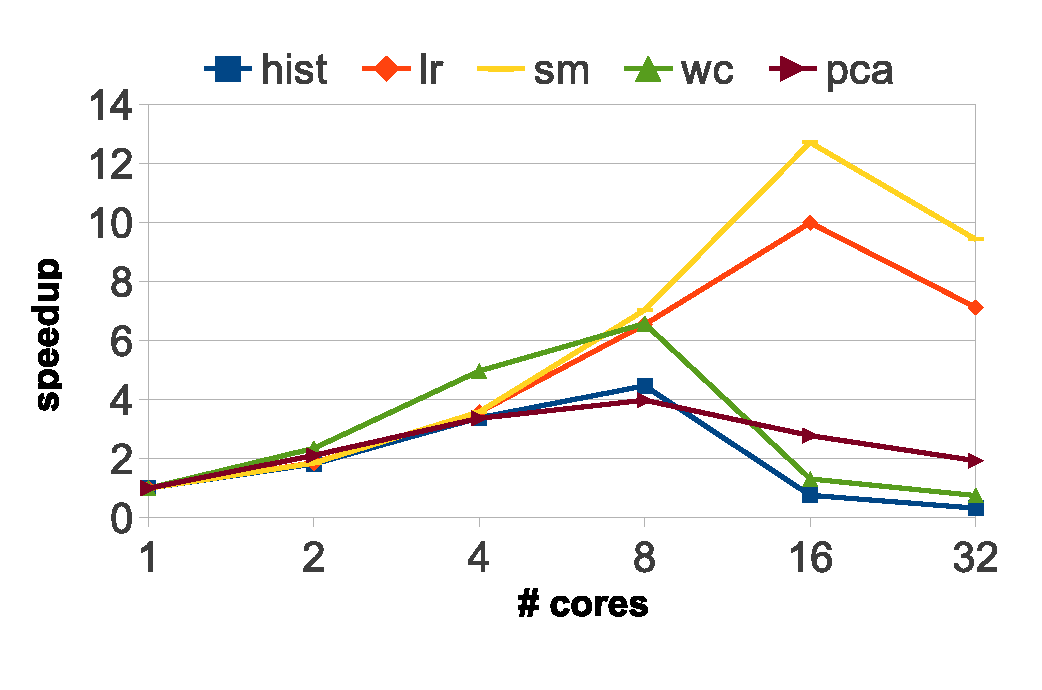
\includegraphics[width=0.45\textwidth]{eps/phoenix_speedup.eps}
	\caption{speedup of Phoenix}
	\label{fig:phoenix:speedup}
\end{figure}

%as depicted in
As shown in this figure \ref{fig:phoenix:speedup}, 
%when using no more than eight cores, the Phoenix scales well on hist ... ;
%when using no more than 16 cores, the Phoenix scales well on sm and le.
the Phoenix scales well on histgram (hist), wordcount (wc) and pca when the number of core is less than 8.
As for the linear\_regression (lr) and string\_match (sm), 
Phoenix performs well with no more than 16 cores.
However, when core number is more than  8, 
the speedup of Phoenix  on hist,  wc and pca is degraded.
For lr and sm, the speedup is degraded when cores is greater than 16.
%For linear\_regression (lr) and string\_match (sm),  using 16 or more  cores leads to speedup degradation.
